\section{Исследовательская часть}

\subsection{Технические характеристики}

Технические характеристики устройства, на котором выполнялся замерный эксперимент:
\begin{itemize}[label*=---]
	\item операционная система Windows 11;
	\item память 16 ГБ;
	\item процессор 3,6 ГГц 6-ядерный процессор AMD Ryzen 5000 series 5.
\end{itemize}

Замеры проводились на ноутбуке, включенном в сеть электропитания. 
Во время тестирования ноутбук был нагружен только интегрированной средой разработки и непосредственно выполняемой программой.

\subsection{Пример работы программы}

На рисунке \ref{fig:example} представлен пример работы программы. 

\begin{figure}
	\centering
	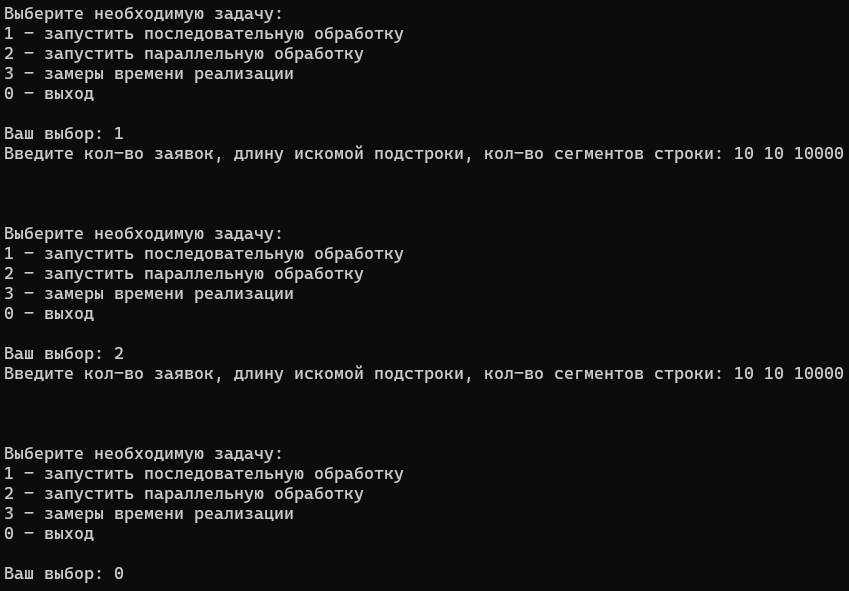
\includegraphics[width=0.4\linewidth]{images/example}
	\caption{Пример работы программы}
	\label{fig:example}
\end{figure}

\newpage

\subsection{Время выполнения реализованных алгоритмов}
Функция perf\_counter из библиотеки time~\cite{time} возвращает время в секундах --- значение типа float.
Является самым точным методом замера коротких промежутков времени~\cite{perf}.

Замеры проводились 100 раз для матриц стоимостей, заполненных случайным образом, размером от 2 до 10.

Результаты измерения времени приведены на рисунке \ref{fig:results}.
\begin{figure}
	\centering
	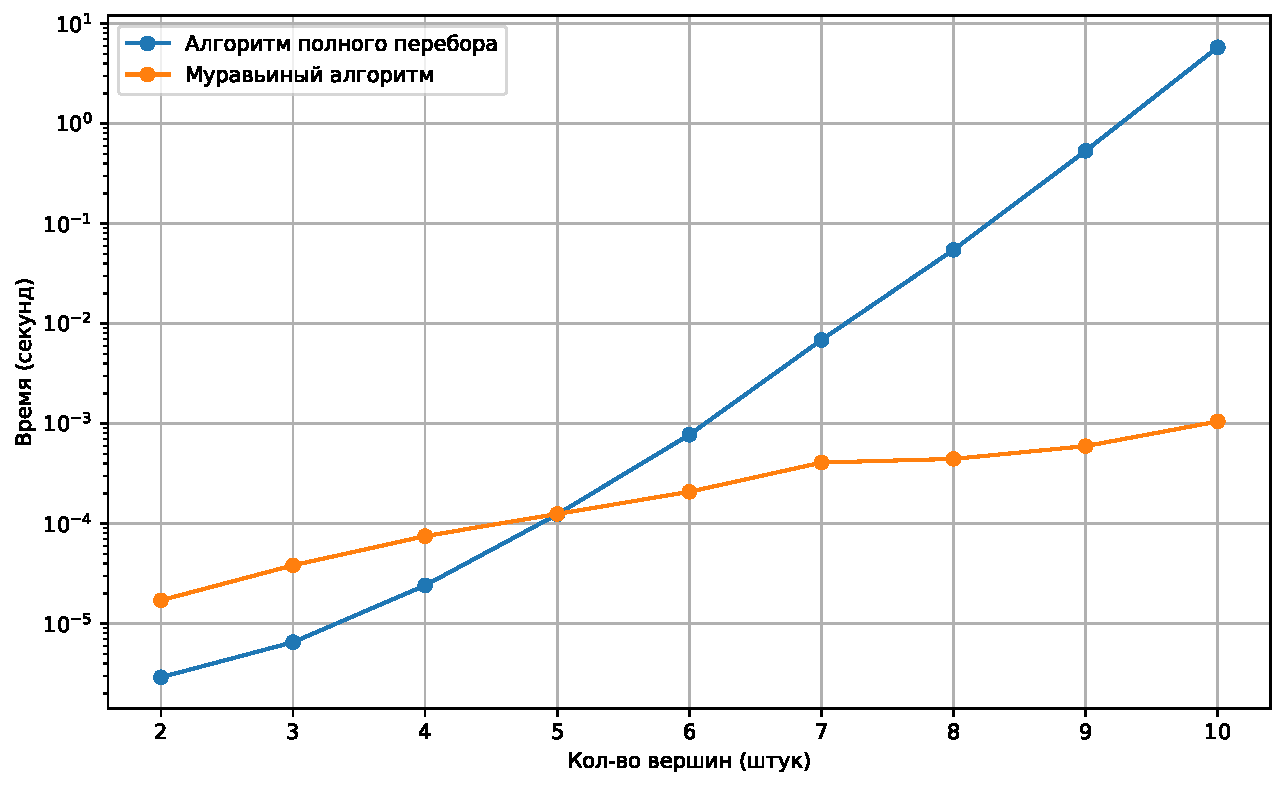
\includegraphics[width=0.7\linewidth]{../src/lab_06/results_logscale}
	\caption{Время выполнения алгоритмов}
	\label{fig:results}
\end{figure}


\subsection{Параметризация}
Целью проведения параметризации является определение таких комбинаций параметров, при которых муравьиный алгоритм дает наилучшие результаты.

В результате автоматической параметризации будет получена таблица со следующими столбцами:
\begin{itemize}[label*={---}]
	\item коэффициент видимости $\alpha$ --- изменяющийся параметр;
	\item коэффициент испарения феромона $\rho$ --- изменяющийся параметр;
	\item число дней/итераций $days$ --- изменяющийся параметр;
	\item эталонный результат $ideal$;
	\item ошибка (разница) $mistake$ между действительным значением и эталонным.
\end{itemize}


\subsubsection{Класс данных}

Класс данных представляет собой набор из трёх матриц стоимостей в диапазоне от 1 до 10 для 10 вершин:

\begin{equation}
	\label{eq:new_matrix1}
	M_{1} = \begin{pmatrix}
		0 & 1 & 2 & 6 & 6 & 6 & 9 & 2 & 5 & 3 \\
		3 & 0 & 4 & 9 & 5 & 6 & 2 & 2 & 8 & 6 \\
		1 & 1 & 0 & 5 & 7 & 8 & 1 & 5 & 4 & 6 \\
		4 & 2 & 1 & 0 & 9 & 5 & 1 & 6 & 7 & 4 \\
		2 & 6 & 3 & 4 & 0 & 6 & 3 & 2 & 3 & 6 \\
		8 & 9 & 4 & 1 & 1 & 0 & 2 & 2 & 7 & 3 \\
		5 & 5 & 3 & 1 & 7 & 1 & 0 & 8 & 8 & 3 \\
		8 & 5 & 1 & 6 & 5 & 7 & 3 & 0 & 6 & 9 \\
		6 & 3 & 4 & 5 & 3 & 8 & 7 & 2 & 0 & 6 \\
		2 & 1 & 3 & 6 & 7 & 7 & 6 & 3 & 3 & 0 \\
	\end{pmatrix}
\end{equation}

\begin{equation}
	\label{eq:new_matrix2}
	M_{2} = \begin{pmatrix}
		0 & 6 & 1 & 4 & 3 & 8 & 1 & 8 & 9 & 1 \\
		2 & 0 & 2 & 9 & 4 & 1 & 6 & 3 & 6 & 2 \\
		8 & 8 & 0 & 2 & 9 & 5 & 1 & 3 & 8 & 7 \\
		2 & 4 & 7 & 0 & 2 & 6 & 1 & 3 & 8 & 8 \\
		2 & 3 & 1 & 9 & 0 & 2 & 8 & 6 & 5 & 5 \\
		2 & 7 & 2 & 3 & 5 & 0 & 5 & 8 & 2 & 7 \\
		7 & 9 & 1 & 1 & 2 & 6 & 0 & 3 & 5 & 9 \\
		3 & 7 & 7 & 2 & 4 & 7 & 4 & 0 & 6 & 8 \\
		4 & 9 & 6 & 8 & 6 & 6 & 4 & 7 & 0 & 5 \\
		8 & 8 & 9 & 4 & 8 & 2 & 3 & 9 & 8 & 0 \\
	\end{pmatrix}
\end{equation}

\begin{equation}
	\label{eq:new_matrix3}
	M_{3} = \begin{pmatrix}
		0 & 6 & 4 & 7 & 4 & 9 & 7 & 4 & 8 & 2 \\
		7 & 0 & 7 & 7 & 9 & 9 & 3 & 2 & 2 & 3 \\
		7 & 8 & 0 & 1 & 5 & 2 & 7 & 4 & 5 & 2 \\
		4 & 6 & 9 & 0 & 4 & 2 & 4 & 6 & 6 & 8 \\
		9 & 9 & 7 & 4 & 0 & 2 & 7 & 2 & 7 & 7 \\
		6 & 2 & 8 & 2 & 9 & 0 & 1 & 5 & 4 & 7 \\
		6 & 6 & 5 & 4 & 9 & 1 & 0 & 7 & 4 & 4 \\
		1 & 2 & 4 & 4 & 6 & 3 & 7 & 0 & 4 & 8 \\
		2 & 6 & 3 & 3 & 5 & 9 & 7 & 5 & 0 & 3 \\
		8 & 2 & 3 & 7 & 9 & 4 & 6 & 3 & 7 & 0 \\
	\end{pmatrix}
\end{equation}


Для данного класса данных приведена таблица~\ref{tab:data_comparison} с выборкой 10 параметров, которые наилучшим образом решают поставленную задачу.
Ошибок в среднем --- значение, указывающее на среднюю разницу идеального и найденного оптимального пути во время процесса параметризации класса данных.

\begin{table}[hbtp]
	\centering
	\caption{Результат выборки параметров}
	\label{tab:data_comparison}
	\begin{tabular}{|c|c|c|c|}
		\hline
		\textbf{$\alpha$} & {$\rho$} & {Итерации, шт.} & {Среднее значение ошибки} \\
		\hline
		0.4 & 0.2 & 300 & 0 \\
		0.4 & 0.7 & 300 & 0 \\
		0.7 & 0.7 & 300 & 0 \\
		0.7 & 0.7 & 500 & 0 \\
		0.1 & 0.3 & 300 & 0 \\
		0.1 & 0.4 & 400 & 0.333 \\
		0.1 & 0.9 & 500 & 0.333 \\
		0.2 & 0.1 & 200 & 0.333 \\
		0.2 & 0.3 & 500 & 0.333 \\
		0.3 & 0.1 & 500 & 0.333 \\
		\hline
	\end{tabular}
\end{table}
